\subsection*{Généralités}
\textbf{Notations:}
\begin{align*}
    \frac{\partial u}{\partial y}     & = u_y    & \frac{\partial^2 u}{\partial y^2}         & = u_{yy} \\
    \frac{\partial^2 u}{\partial x^2} & = u_{xx} & \frac{\partial^2 u}{\partial x\partial y} & = u_{xy}
\end{align*}
\textbf{Condition de linéarité:}
\begin{subequations}
    \begin{equation*}
        \mathcal{L}(u+v)=\mathcal{L}(u)+\mathcal{L}(v)
    \end{equation*}
    \begin{equation*}
        \mathcal{L}(cu)=c\mathcal{L}(u)
    \end{equation*}
\end{subequations}
Si $\mathcal{L}u=0$ : \textit{linéaire homogène} \\
Si $\mathcal{L}u=f$ : \textit{linéaire inhomogène}\\
\textbf{Divergence:}\\
Pour un champ vectorielle $\overrightarrow{v}(x,y,z)=\begin{pmatrix} v_1(x,y,z) \\ v_2(x,y,z) \\ v_3(x,y,z) \end{pmatrix}$:
\begin{equation*}
    \text{div}(\overrightarrow{v})=\nabla\cdot\overrightarrow{v}=\frac{\partial v_1}{\partial x}+\frac{\partial v_2}{\partial y}+\frac{\partial v_3}{\partial z}
\end{equation*}
\textbf{Gradient:}\\
Pour un champ scalaire $u(x,y,z)$:
\begin{equation*}
    \text{grad}(u)=\nabla u=\begin{pmatrix} \frac{\partial u}{\partial x} \\ \frac{\partial u}{\partial y} \\ \frac{\partial u}{\partial z} \end{pmatrix}
\end{equation*}
\textbf{Rotationnel:}\\
\begin{equation*}
    \text{curl}(\overrightarrow{v}) = \nabla \times \overrightarrow{v} =
    \begin{pmatrix}
        \frac{\partial}{\partial x} \\
        \frac{\partial}{\partial y} \\
        \frac{\partial}{\partial z}
    \end{pmatrix}
    \times
    \begin{pmatrix}
        v_1(x,y,z) \\
        v_2(x,y,z) \\
        v_3(x,y,z)
    \end{pmatrix}
    =
    \begin{pmatrix}
        \frac{\partial v_3}{\partial y} - \frac{\partial v_2}{\partial z} \\
        \frac{\partial v_1}{\partial z} - \frac{\partial v_3}{\partial x} \\
        \frac{\partial v_2}{\partial x} - \frac{\partial v_1}{\partial y}
    \end{pmatrix}
\end{equation*}
\textbf{Laplacien}:
\begin{equation*}
    \Delta u=\text{div}(\Delta u)=u_{xx}+u_{yy}+u_{zz}
\end{equation*}
\textbf{Quelques propriétés:}
\begin{equation*}
    \text{div}(u\cdot \overrightarrow{v})=\overrightarrow{v}\cdot\nabla u+u\cdot\text{div}(\overrightarrow{v})
\end{equation*}
\textbf{Conditions initiales et aux bords:}\\
$u(x,t_0)=\phi(x)$ (diffusion, flux de chaleur)\\
$u(x,t_0)=\phi(x)$ et $u_t(x,t_0)=\psi(x)$ (ondes)\\
$u$ est spécifié : \textit{Dirichlet}\\
$\frac{\partial u}{\partial n}$ est spécifié : \textit{Neumann}\\
$\alpha u+\beta\frac{\partial u}{\partial n}$ est spécifié : \textit{Robin}\\
\textbf{Quelques types d'EDO:}\\
\underline{Equation de transport:}
\begin{equation*}
    u_t+cu_x=0
\end{equation*}
\underline{Equation d'onde:}\\
Pour une onde se propageant dans la direction $x$:
\begin{equation*}
    u_{tt}=c^2u_{xx}
\end{equation*}\\
Pour une onde se propageant dans deux directions:
\begin{equation*}
    u_{tt}=c^2\Delta u=c^2(u_{xx}+u_{yy})
\end{equation*}
\underline{Equation de diffusion:}
\begin{equation*}
    u_t=ku_{xx}
\end{equation*}
\textbf{EDO connues:}
\begin{equation*}
    \begin{aligned}
         & x''+\beta^2x=0 \quad\rightarrow\quad x=A\cos(\beta t)+B\sin(\beta t) \\
         & x''-\beta^2x=0 \quad\rightarrow\quad x=Ce^{\beta t}+De^{-\beta t}    \\
         & =(C+D)\cosh(\beta t)+(C-D)\sinh(\beta t)                             \\
         & x''=0 \quad\rightarrow\quad x=Et+F                                   \\
         & x'\pm \beta x=0 \quad\rightarrow\quad x=Ge^{\mp\beta t}              \\
    \end{aligned}
\end{equation*}
\textbf{Taylor}\\
\underline{1D:}\\
Le développement de Taylor de $u(x)$ autour de $x_i$:
\begin{equation*}
    u(x)=u(x_i)+\frac{u'(x_i)}{1!}(x-x_i)+\frac{u''(x_i)}{2!}(x-x_i)^2+\frac{u'''(x_i)}{3!}(x-x_i)^3+\cdots
\end{equation*}
\underline{2D:}\\
Le développement de Taylor de $u(x,y)$ autour de $(x_i,y_i)$:
\begin{equation*}
    \begin{aligned}
        u(x,y) & =u(x_i,y_i)+(u_x+u_y)(x-x_i,y-y_i)                                     \\
               & +\frac{1}{2!}(u_{xx}+2u_{xy}+u_{yy})(x-x_i,y-y_i)^2                    \\
               & +\frac{1}{3!}(u_{xxx}+3u_{xxy}+3u_{xyy}+u_{yyy})(x-x_i,y-y_i)^3+\cdots
    \end{aligned}
\end{equation*}
\textbf{Max-norm:}
\begin{equation*}
    ||u||_{\infty}=\max_{x\in\Omega}|u(x)|
\end{equation*}


\columnbreak
\subsection*{EDP linéaire du premier ordre}
\textbf{Quelques équations simples:}
\begin{figure}[H]
    \centering
    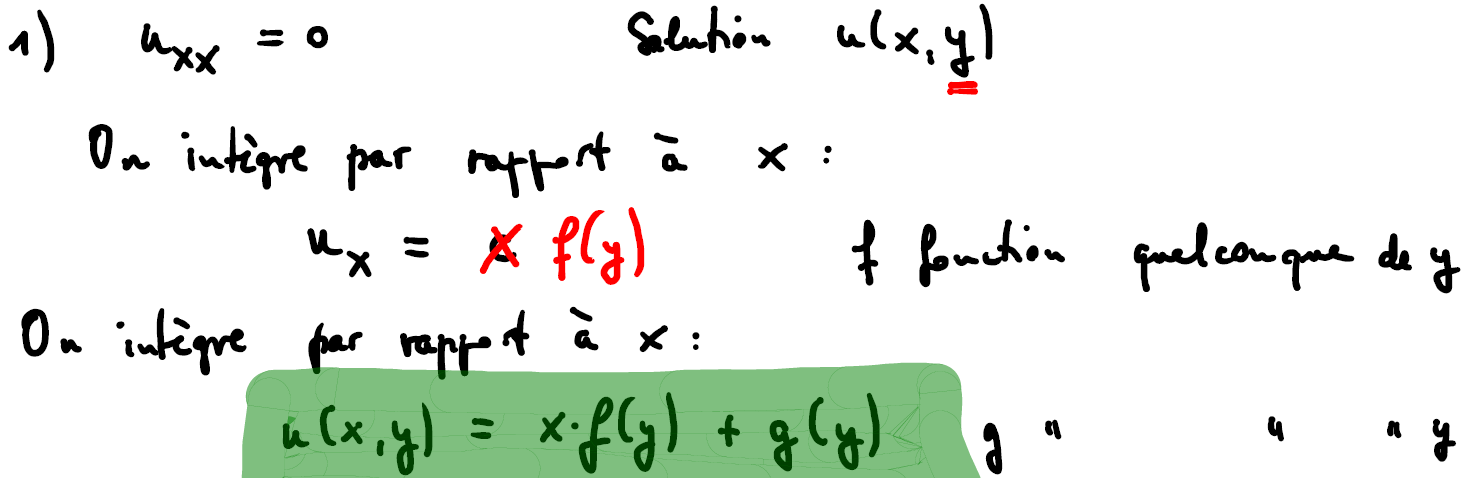
\includegraphics[width=\linewidth]{images/semain1_equ_simple1.png}
\end{figure}
\begin{figure}[H]
    \centering
    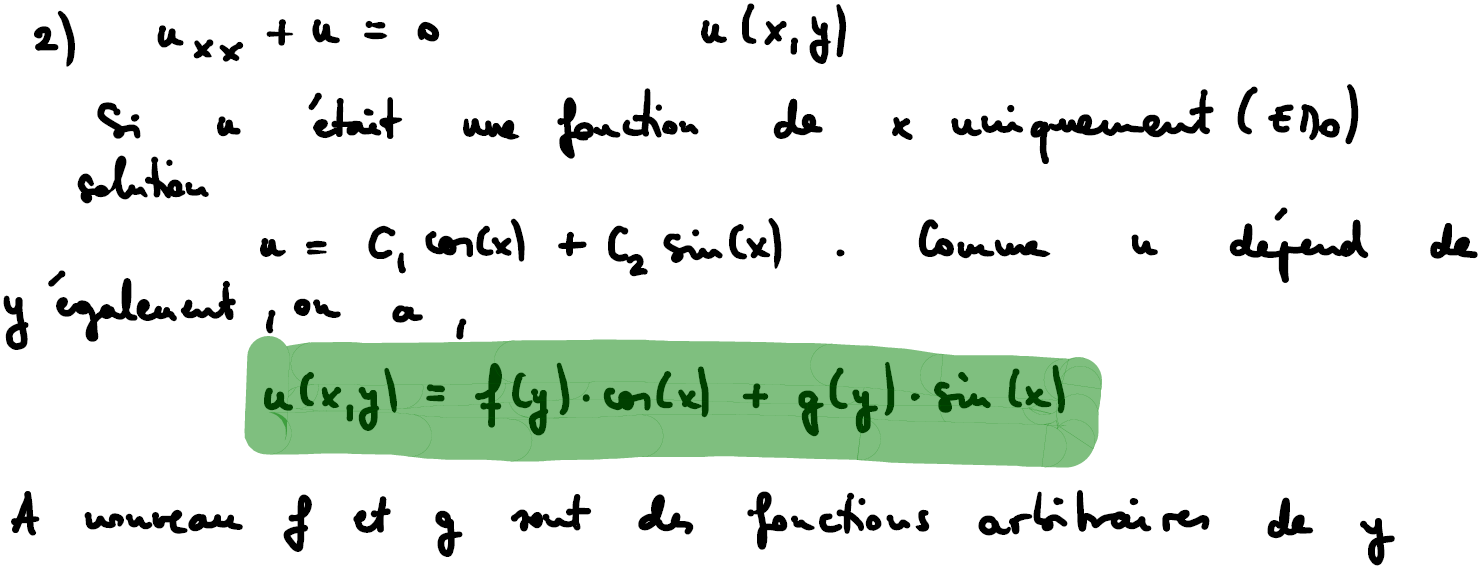
\includegraphics[width=\linewidth]{images/semain1_equ_simple2.png}
\end{figure}
\begin{figure}[H]
    \centering
    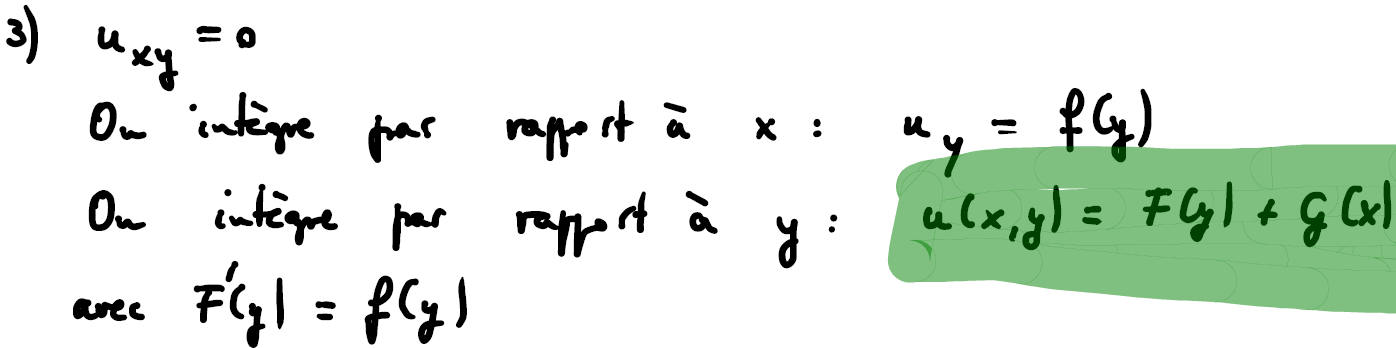
\includegraphics[width=\linewidth]{images/semain1_equ_simple3.png}
\end{figure}
\textbf{Equation à coefficients constants:}
\begin{subequations}
    \begin{equation*}
        au_x+bu_y=0
    \end{equation*}
    \begin{equation*}
        \boxed{u(x,y)=f(bx-ay)}
    \end{equation*}
\end{subequations}
\begin{figure}[H]
    \centering
    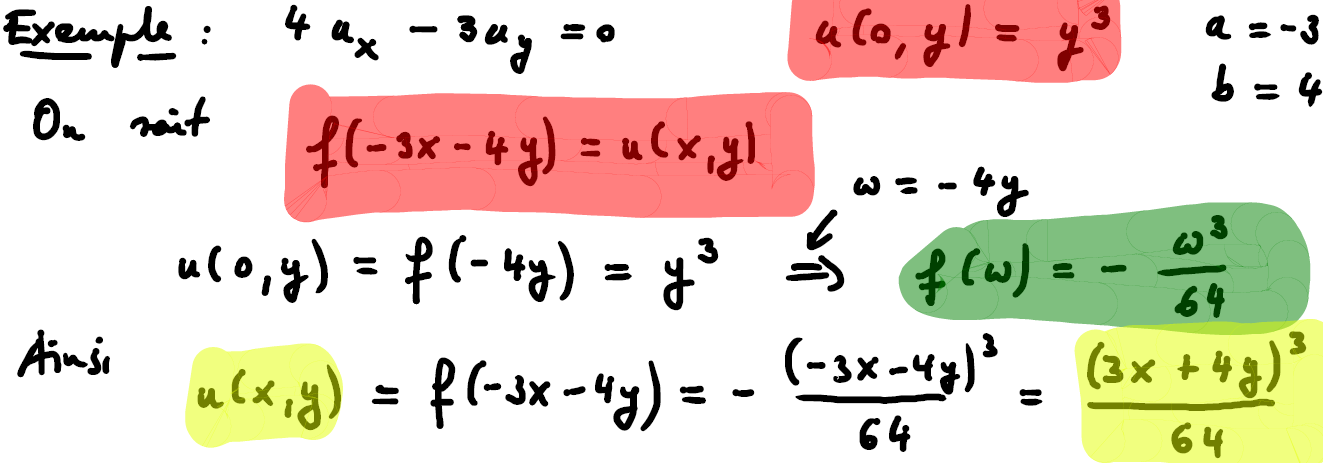
\includegraphics[width=\linewidth]{images/semaine1_equ_coeff_const.png}
\end{figure}
\textbf{Equation à coefficients variables:}
\begin{subequations}
    \begin{equation*}
        a(x,y)u_x+b(x,y)u_y=0
    \end{equation*}
    \begin{equation*}
        \boxed{\frac{\mathrm{d} y}{\mathrm{d} x}=\frac{b(x,y)}{a(x,y)}}
    \end{equation*}
\end{subequations}
\begin{figure}[H]
    \centering
    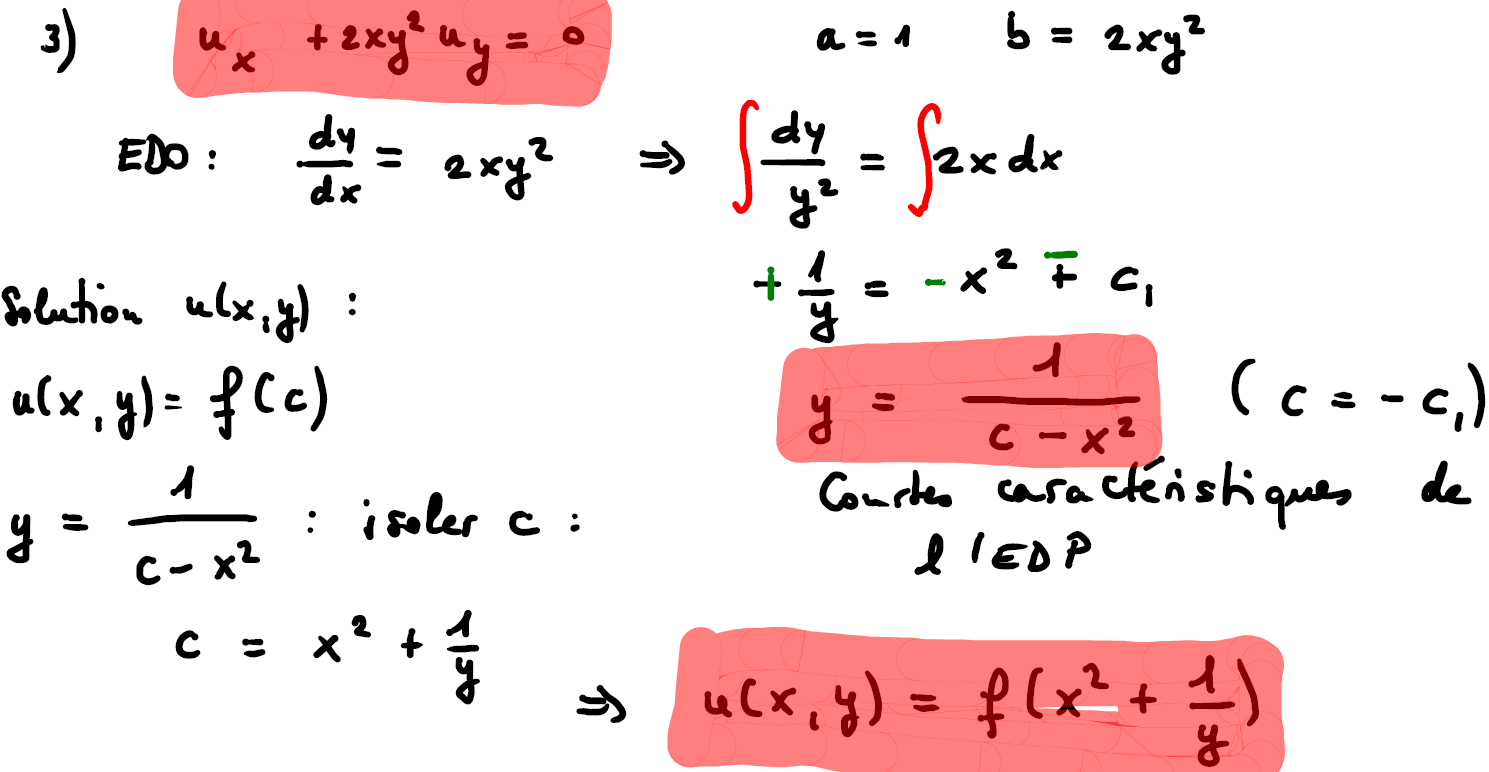
\includegraphics[width=\linewidth]{images/semaine1_equ_coeff_var1.png}
\end{figure}



\subsection*{EDP linéaire du second ordre}
\begin{equation*}
    Au_{xx}+Bu_{xy}+Cu_{yy}+Du_x+Eu_y+Fu=G
\end{equation*}
$A$, $B$, $C$, $D$, $E$, $F$, $G$ constantes ou des fonctions de $x$ et $y$.\\
\textit{Parabolique} si $B^2-4AC=0$\\
\textit{Hyperbolique} si $B^2-4AC>0$\\
\textit{Elliptique} si $B^2-4AC<0$\\
Trouver les régions de l'EDP:
\begin{equation*}
    yu_{xx}-2u_{xy}+xu_{yy}=0
\end{equation*}
\begin{figure}[H]
    \centering
    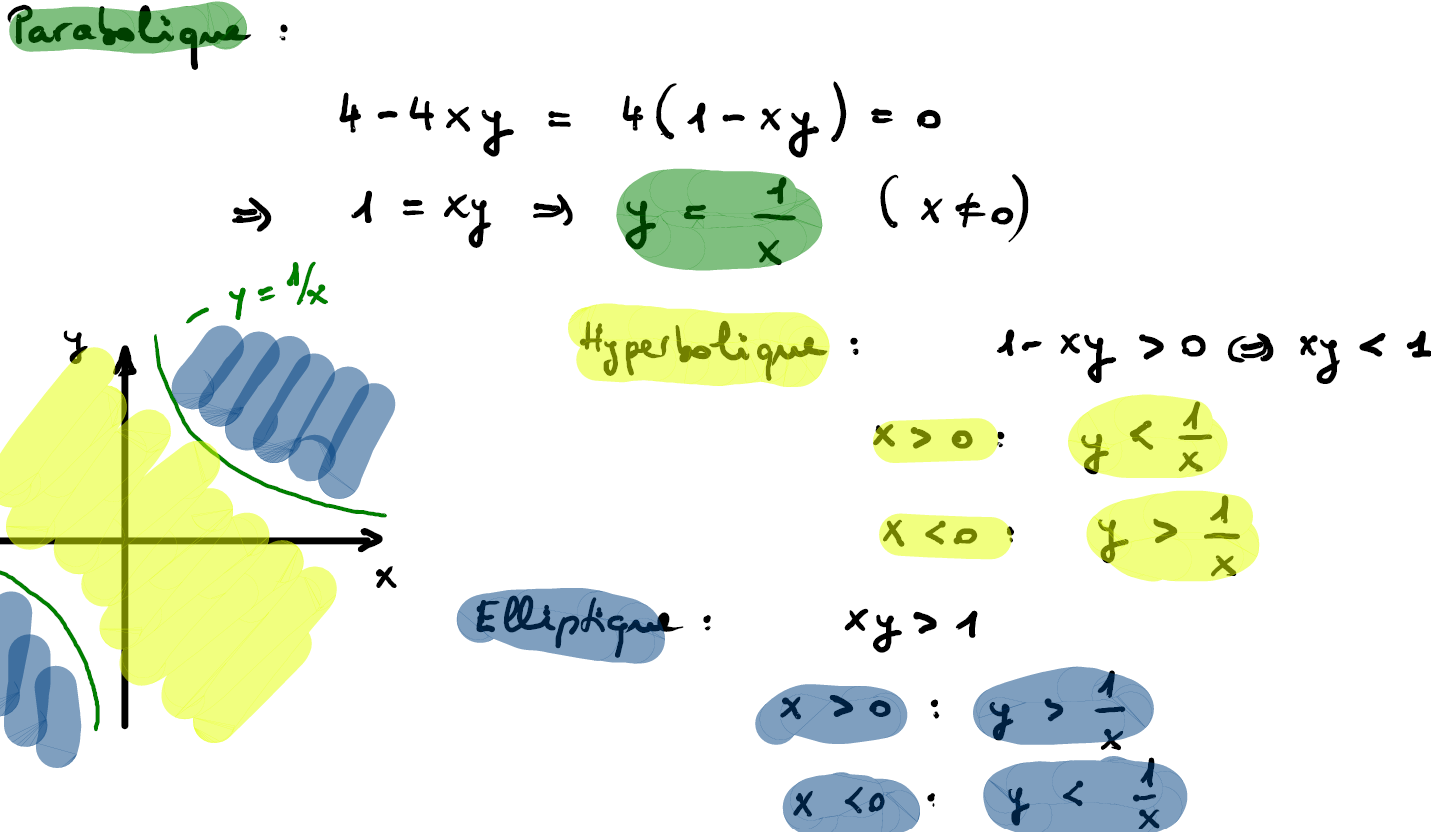
\includegraphics[width=\linewidth]{images/semaine2_edp_ordre2_classif.png}
\end{figure}



